\documentclass{sigchi}

% Use this command to override the default ACM copyright statement (e.g. for preprints). 
% Consult the conference website for the camera-ready copyright statement.
\toappear{
For permission to redistribute copies of this paper, in digital or print media form,
please contact the authors listed above --- Galen Weld (gcw33@cornell.edu) and Kevin Guo (kg344@cornell.edu)\\
\\
{\confname{Final Project paper for Cornell INFO 4120}}\\
May 10, 2017, Cornell University, Ithaca, New York.\\
Copyright 2017.
}

% Arabic page numbers for submission. 
% Remove this line to eliminate page numbers for the camera ready copy
%\pagenumbering{arabic}


% Load basic packages
\usepackage{balance}  % to better equalize the last page
\usepackage{graphics} % for EPS, load graphicx instead
\usepackage{times}    % comment if you want LaTeX's default font
\usepackage{url}      % llt: nicely formatted URLs
\usepackage{array}	  % array: for tables
\usepackage[labelfont=bf]{caption}

% llt: Define a global style for URLs, rather that the default one
\makeatletter
\def\url@leostyle{%
  \@ifundefined{selectfont}{\def\UrlFont{\sf}}{\def\UrlFont{\small\bf\ttfamily}}}
\makeatother
\urlstyle{leo}


% To make various LaTeX processors do the right thing with page size.
\def\pprw{8.5in}
\def\pprh{11in}
\special{papersize=\pprw,\pprh}
\setlength{\paperwidth}{\pprw}
\setlength{\paperheight}{\pprh}
\setlength{\pdfpagewidth}{\pprw}
\setlength{\pdfpageheight}{\pprh}

% Make sure hyperref comes last of your loaded packages, 
% to give it a fighting chance of not being over-written, 
% since its job is to redefine many LaTeX commands.
\usepackage[pdftex]{hyperref}
\hypersetup{
pdftitle={SIGCHI Conference Proceedings Format},
pdfauthor={LaTeX},
pdfkeywords={SIGCHI, proceedings, archival format},
bookmarksnumbered,
pdfstartview={FitH},
colorlinks,
citecolor=black,
filecolor=black,
linkcolor=black,
urlcolor=black,
breaklinks=true,
}

% create a shortcut to typeset table headings
\newcommand\tabhead[1]{\small\textbf{#1}}


% End of preamble. Here comes the document.
\begin{document}

\title{SmartBag: Intelligent Medication and Equipment Management for EMS
	Providers}

\numberofauthors{2}
\author{
  \alignauthor Galen Weld\\
    \affaddr{Cornell University}\\
    \affaddr{Computer Science}\\
    \email{gcw33@cornell.edu}\\
    \affaddr{(206) 588-5370}
  \alignauthor Kevin Guo\\
    \affaddr{Cornell University}\\
    \affaddr{Information Science}\\
    \email{kg344@cornell.edu}\\
    \affaddr{(908) 601-8030}
}

\maketitle

\begin{abstract} \label{abstract}

EMS Care Providers are faced with a large number of tedious tasks which
detract from their primary role of providing lifesaving patient care.
Daily truck checks and resupply between calls occupy as much as 10\% of
a 12 hour shift,~\cite{checks} and are absolutely critical to providing
quality care, yet compliance with equipment check procedures is frequently
poor. We present SmartBag, an intelligent medication and equipment management
system, to automate the equipment management process and allow care
providers to focus on their primary task.

\end{abstract}

\keywords{
	emergency medicine; emergency medical services; inventory management; 
    medication; medication management; medication preservation; cognitive load
    reduction; automation.
}


\section{Introduction} \label{intro}
Accurate inventory management is critical to quality pre-hospital emergency
medical care. A piece of equipment may stay unused in a bag or vehicle for
months, but care providers still need to access it at a moment’s notice,
and be confident that it is still functional. Current management practices
are essentially unchanged since the advent of ambulance services, the only
distinction is that modern paramedics have even more equipment that they
must manage - a modern ambulance may have more than 500 items on-board! ~\cite{rfid}

The current widespread practice is for crews to perform a daily truck check,
and then resupply items between calls as needed. However, this approach
has numerous drawbacks - truck checks are tedious and are often rushed or not
performed in their entirety, despite policies mandating them. Even when a truck
check is performed, accuracy is often poor, and only a single missed item is
enough to possibly cause a critical failure. On busy shifts, when crews respond
from one call directly to another, without an opportunity to return to the station
to resupply, it is frequently difficult for EMS crews to track which items are
missing while simultaneously managing patient care and operational concerns such
as radio traffic.

These issues offer a clear space for a technological solution - computerized
systems are far better than humans at performing repetitive, tedious tasks,
and they never lose interest or forget to do their job. For this reason, we developed
SmartBag, which performs much of the work of inventory management and equipment
checks in the background, so that EMS staff can focus on their primary task ---
providing quality patient care in emergent situations.


\section{Background} \label{background}
The process of checking supplies is a regular part of the job for emergency medical
personnel. Unlike hospitals or clinics, where supplies are often tracked with
sophisticated electronic inventory systems, most supplies for ambulances and other
first response vehicles are tracked manually through paper checklists. This is a
tedious and error-prone process that can lead to equipment being missing from
ambulances during calls. Such lapses in inventory have caused response times to
increase and even lead to multiple unnecessary downgrades to the response of
critical calls~\cite{response}. The lack of precise temperature readings and control
in most emergency vehicles also has lead to problems where temperature-sensitive
medications have become unusable before their labeled expiration dates~\cite{drugs}.

\section{Motivation} \label{motivation}
By now, it should be clear that equipment management is critical to the safe
functioning of any emergency medical services agency, and a crucial component
of the delivery of quality patient care. Yet as the previous section illustrated,
the importance of thorough equipment checks is often overlooked by EMS employees,
who tend to be more passionate about caring for patients than performing truck
check.

The motivation for developing SmartBag stems from this observation, as well
as the observation that computers are far more suited to performing repetitive,
tedious tasks such as truck check than humans are. Computers don't get bored,
don't get distracted partway through a job, and are happy to work 24/7.

A quality automated equipment management system would take care of the tedious,
and unglamorous aspects of emergency medicine, automating repetitive tasks such
as daily equipment checks, monitoring expiration dates and temperature limits,
tracking which items are used on a call and need to be resupplied, etc --- and
do all of this in the background, without interfering with the usability of the
bag, thusly allowing care providers to focus on their primary responsibility of
providing quality patient care.


\subsection{System Goals} \label{goals}
With the preceding motivating factors in mind, we were then able to begin
formulating in greater detail what functions our system should provide,
and which features were most critical. After discussing with EMS providers
at Cornell University EMS~\cite{cuems}, the following list of criteria for
a successful equipment management system were developed:

\begin{enumerate}
\item \label{goal:focus}
	Offload the cognitive load of equipment management from
	care providers,	to allow them to focus on their primary tasks.

\item \label{goal:access}
	Provide an easy-to-use interface which will not impede
	access to gear in emergent situations.

\item \label{goal:accuracy}
	Accurately and automatically track the environmental
	constraints of medications and	supplies, including temperature limits
    and expiration dates.

\item \label{goal:safety}
	Notify users of expired, damaged, or missing equipment
	to prevent compromised care.

\item \label{goal:exchange}
	Allow seamless exchange of items between multiple bags.
\end{enumerate}

These goals for a successful system enabled us to begin to design in
detail the functionality of our prototype system.


\section{Prototype Design} \label{design}
From the beginning, it was clear that the system would need to be robust,
self-contained, consume minimal electricity, and easy to use. To achieve
these goals, we decided to construct a system around inexpensive,
disposable RFID tags which can be read contactlessly from a distance of up
to several inches. RFID tags have approximately 1 kilobyte worth of onboard
storage, which enables the details of the associated item to be written
directly to the tag itself. This has two major advantages – firstly, it adds
redundancy by removing the need for complex, centralized database mapping
medication information to tags. Secondly, and more importantly, this enables
items to be seamlessly transfered from one bag to another, without needing to
keep the two bags in sync --- allowing us to achieve goal~\ref{goal:exchange}.

\begin{figure}[!ht]
\centering
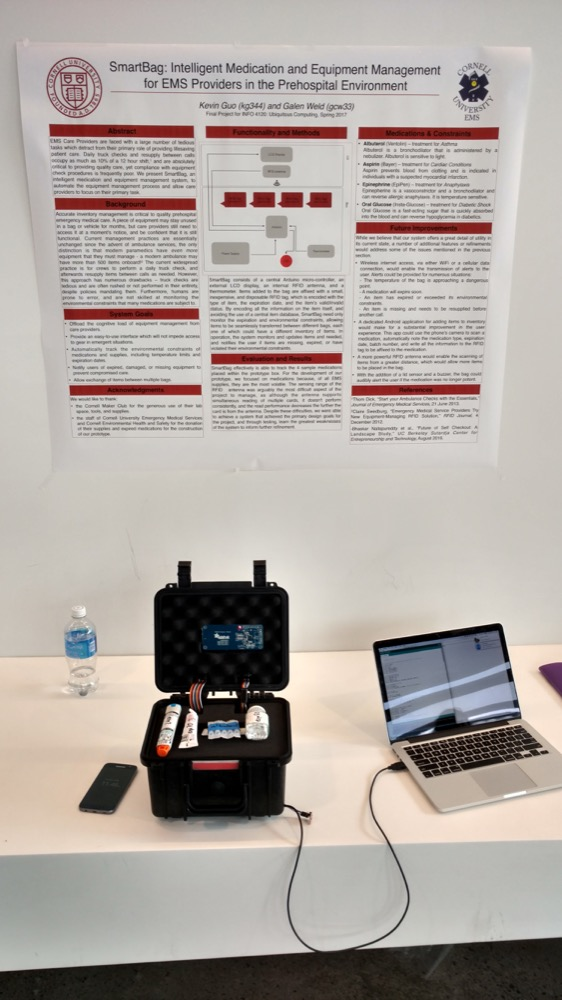
\includegraphics[width=\columnwidth]{demo}
\caption{The completed prototype and demo, as displayed at UbiComp final
	project	demo day at Gates Hall, 4 May 2017.}
\label{fig:demo}
\end{figure}

For the first prototype described here, we elected to limit the scope of the
project to that of a system that simply focuses on tracking medications, not
other first-aid supplies. The decision to focus only on medications vastly
reduces the number of items which need to be monitored, making the system more
straightforward to develop and debug. Medications are arguably the most important
items to monitor, as they are used less frequently but are absolutely critical
to patient care when they are needed. Furthermore, medications are also subject
to more constraints than other first aid supplies. Unlike items such as gauze or
splinting materials, medications have expiration dates, and many are subject to
environmental restrictions (such as a limited temperature range or limited
exposure to light) in order to ensure potency. Finally, medications are also
some of the more valuable items in a typical EMS bag, and as such, it makes
a medication monitoring system perhaps more economically viable.

To store these medications and the rest of the system, we selected a hard-sided,
waterproof plastic case~\cite{pelicase}. Despite the prototype name implying the
use of a \emph{bag}, a hard-sided case or box offers several advantages. It allows
us to have a more rigid, inflexible enclosure which makes mounting and wiring
electronics more simple. It also does an excellent job of protecting its contents;
not just medications but also power supplies, batteries, and other key components
of the system. While the system could absolutely be adapted to fit inside of a
soft-sided bag or backpack, Pelican-style hardcases such as the one we selected
for SmartBag are ubiquitous in the emergency medical services industry, and it's
not at all difficult to imagine our system being adopted as-is for tracking
medications or other smaller items.

For the "brain" of the system, we opted to use an Arduino Uno~\cite{arduino}.
While the Uno is neither the highest performance nor the most compact embedded
systems microcontroller, the ubiquity of the system and availability of excellent
software libraries and hardware components made it a logical choice. The system
has available for it a pre-assembled RFID breakout~\cite{rfid_breakout} which,
while not the most powerful RFID antenna available, made development
straightforward, a key priority for the construction of our prototype and demo.


\section{Prototype Functionality} \label{functionality}
After the design process, a first prototype was constructed for an initial demo.
The first SmartBag consists of a central Arduino micro-controller, an external
LCD display, an internal RFID antenna, and a thermometer, contained within a
small plastic case. Items added to the bag are affixed with a small, inexpensive,
and disposable RFID tag, which is encoded with the type of item, the expiration
date, and the item’s valid/invalid status. In operation SmartBag continuously
monitors the time, date, and temperature, and constantly updates the user if
items are expired or have lost potency. If a medication is damaged or expired,
SmartBag writes an invalid bit to the medication's RFID tag, so that even if
SmartBag is reset or the medication is transferred to another bag, other systems
will be aware that the medication is no longer valid. When the bad medication is
replaced with  a new, valid medication, SmartBag can immediately detect this,
silence any alarms, and immediately restore itself to a normal condition.


\subsection{Hardware Functionality} \label{hardware}
The prototype was constructed within a hard-sided plastic box~\cite{pelicase},
with two main groupings of components. The lid of the box was embedded with the
RFID~\cite{rfid_breakout} sensor and the 2-row LCD display. A hole was cut into
the lid of the display, and covered with clear acrylic, so the user could view
the display with the box closed.

\begin{figure}[!ht]
\centering
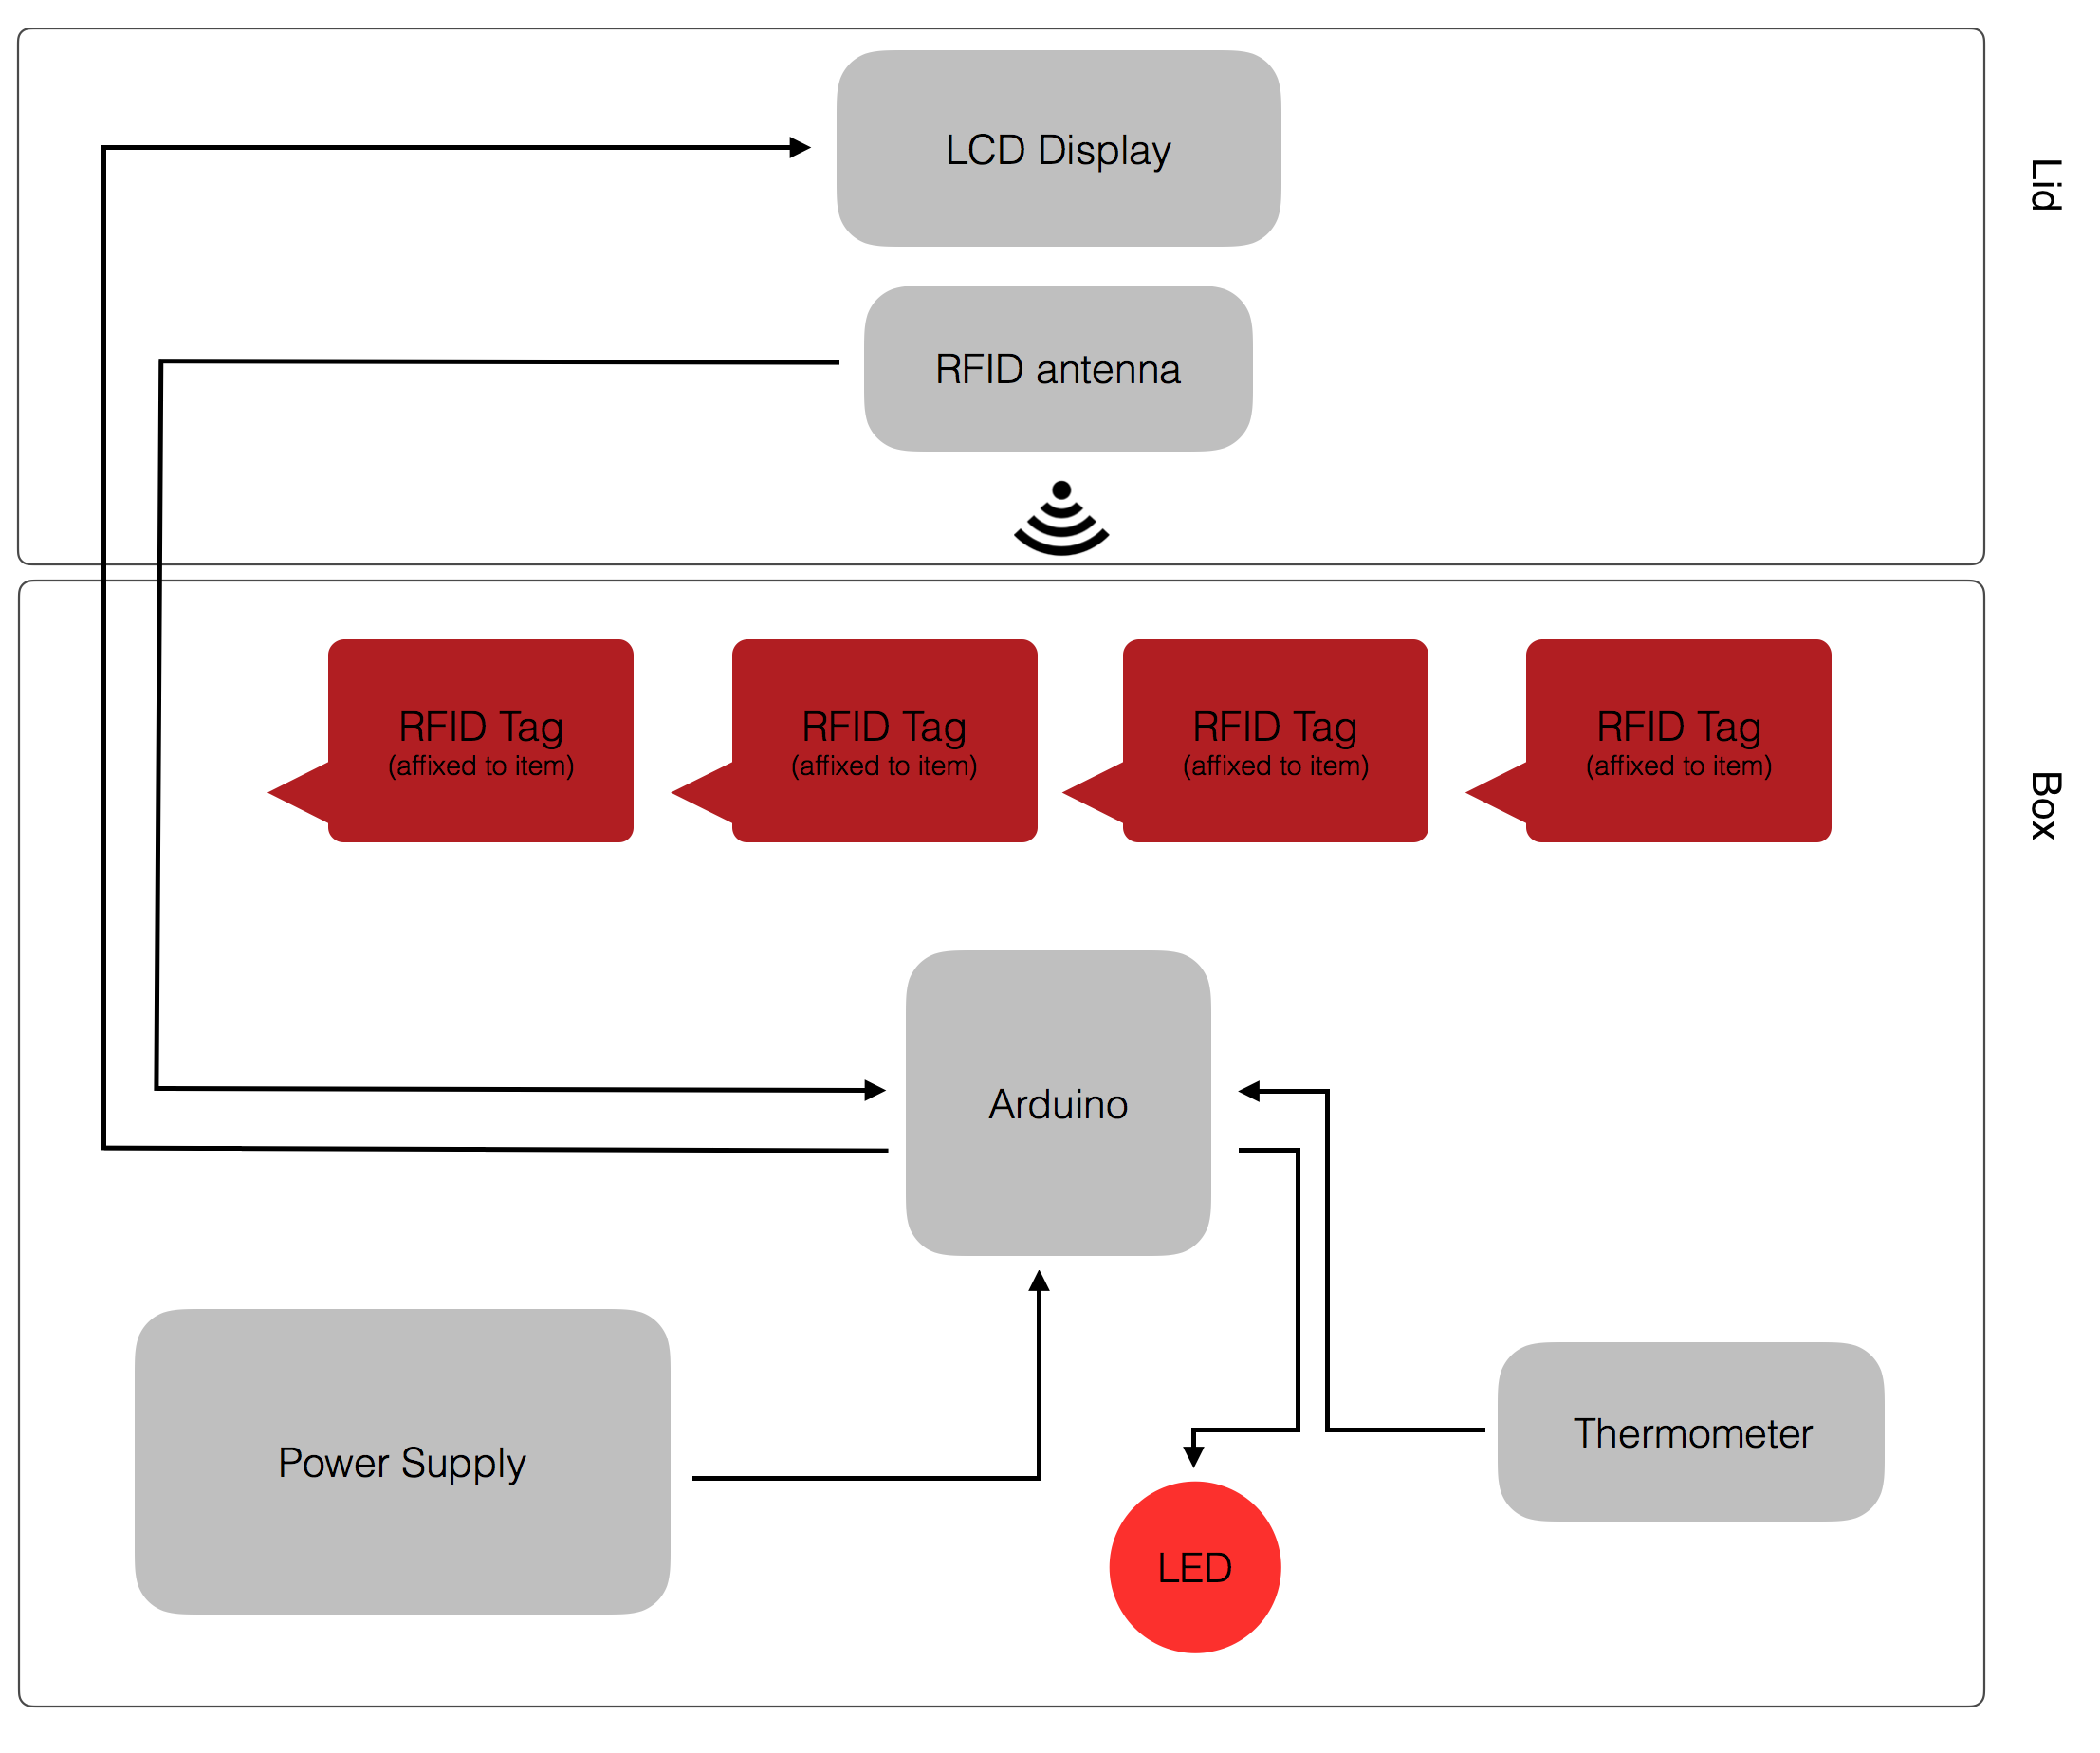
\includegraphics[width=\columnwidth]{system_diagram}
\caption{A visual diagram explaining the interactions between the major
	hardware components of the SmartBag system.}
\label{fig:hardware_diagram}
\end{figure}

Ribbon cables crossed the hinge of the lid, as depicted in
Figure~\ref{fig:final_prototype}, to allow the electronics in the lid to
communicate with the electronics in the main body of the box. Beneath a false
bottom of the box we affixed the Arduino~\cite{arduino} and thermometer. The
components were all assembled and connected using a breadboard, depicted in Figure ~\ref{fig:wiring}, which was attached to the bottom of the box using double-sided
adhesive tape. A hole was added through the side of the box, to connect a USB cable
for power supply and debugging purposes. A diagram of component wiring and
communication is visible in Figure~\ref{fig:hardware_diagram}.

\begin{figure}[!ht]
\centering
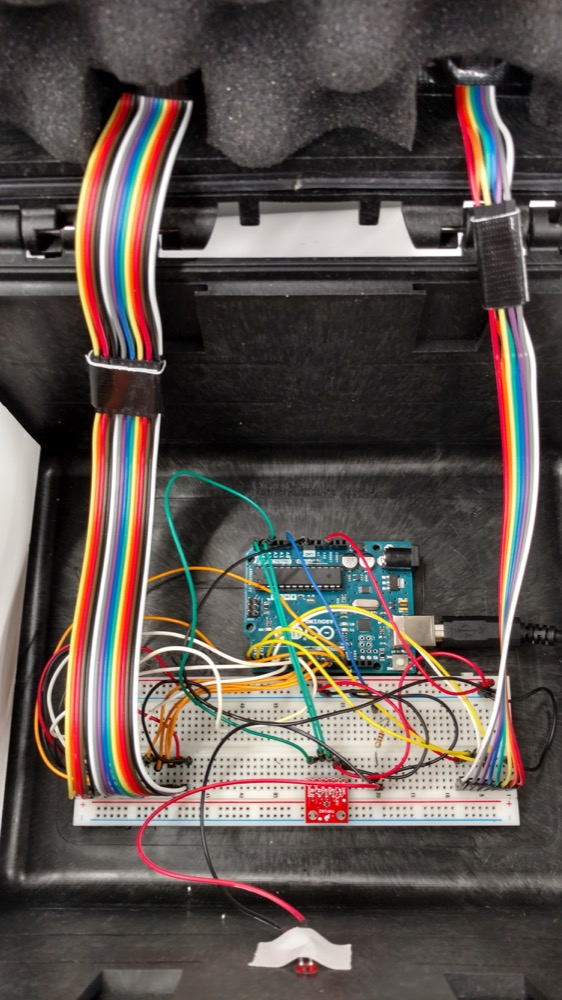
\includegraphics[width=\columnwidth]{box_bottom}
\caption{A close up of the bottom of the box, where most of the major
	electronic components are located and the wiring is. The two ribbon
    cables connect to the RFID sensor and LCD display.}
\label{fig:wiring}
\end{figure}

We covered the false bottom of the box with a sheet of clear acrylic, to
protect the electronics, and then added a thick sheet of configurable
"pick-and-pluck" foam to allow the user to customize the layout of the medications.
The lid of the bag, and the electronics contained within it, were padded with
more foam, as visible in~\ref{fig:final_prototype} to protect the electronics as
well as the medications when the box is closed.

\begin{figure}[!ht]
\centering
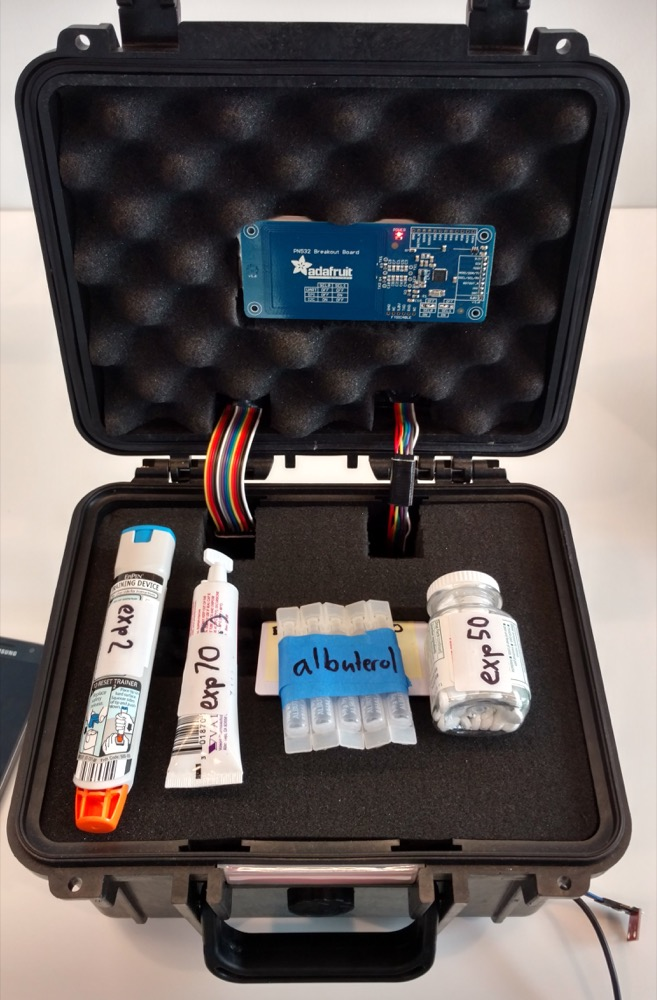
\includegraphics[width=\columnwidth]{final_prototype}
\caption{The final SmartBag prototype, loaded with medications.
	RFID tags are visible on each item, as is the RFID antenna
    embedded in the lid of the bag.}
\label{fig:final_prototype}
\end{figure}

\bigskip
\subsection{Software Functionality} \label{software}
The software for SmartBag, written entirely in the Arduino IDE, was shaped
in large part by the limitations of the Adafruit RFID sensor~\cite{rfid_breakout}
and associated code library, which, by our understanding, required all calls to
the RFID sensor to wait until a card is read until returning from the function
call. This prevented us from implementing the software as initially intended,
because we could not have a main loop body which ran at a constant frequency.

However, by virtue of the fact that when the box is closed, RFID tags are
constantly being scanned, a "close-enough" implication was achieved. After
initializing the hardware components, display, and medication inventory,
the system begins a loop, which is repeated continuously after startup. This
loop is summarized in Figure~\ref{fig:software_diagram} and detailed below.
All of the code described is publicly available on the author's GitHub
page.~\cite{github}

\begin{figure}[!ht]
\centering
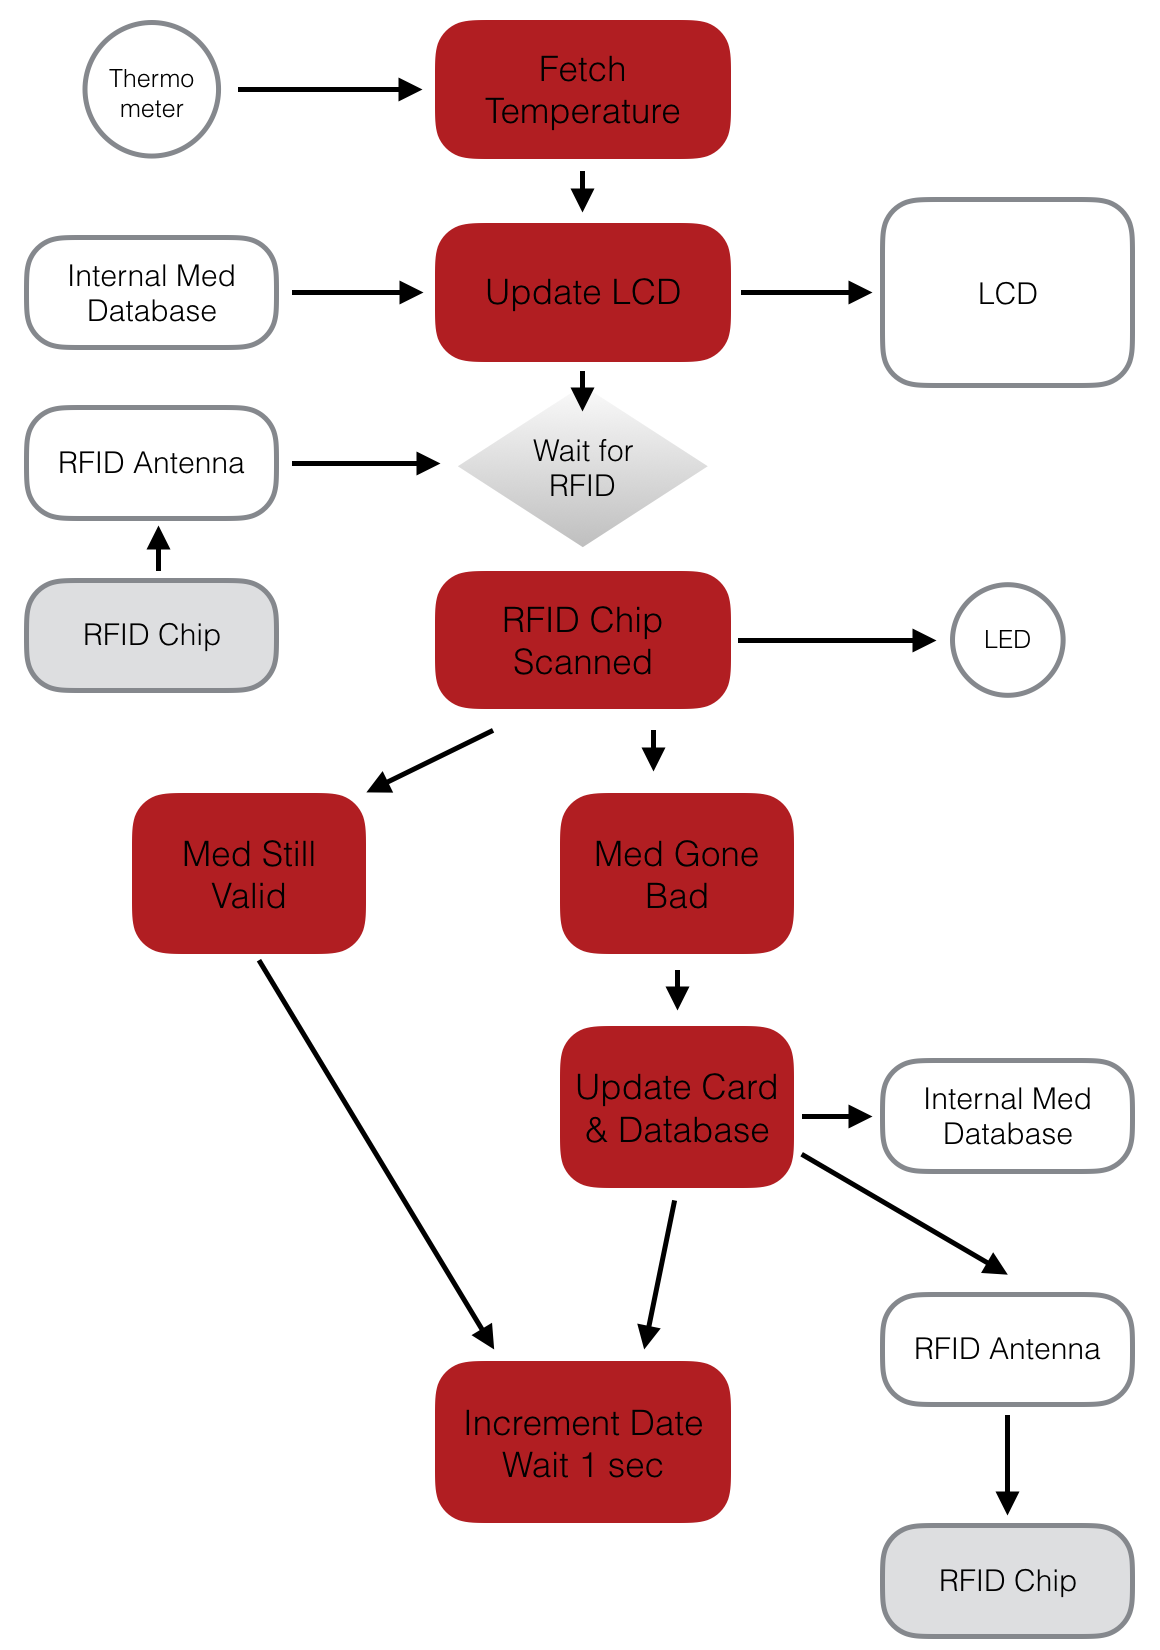
\includegraphics[width=\columnwidth]{software_loop}
\caption{A visual diagram showing the flow of the software components
	of the system as and how they interact with the various hardware
    elements during a single loop of the main code body of the SmartBag
    system.}
\label{fig:software_diagram}
\end{figure}

As mentioned above, an inventory of the medications contained in the system
is created at system startup, and updated continuously during usage. The 
internal inventory database is distinct from the information stored on the
medications' RFID tags, as it is cleared on restart, and only contains
temporary information about the items as a "cache" for the interval between
repeated scans of an item --- a period of only few seconds.

The database contains, for each item in the inventory, only information about
the item's status --- is it present and OK, missing, expired, or exceeded
its temperature constraints. This database is used to update the LCD display
readout at the beginning of each loop.


\subsubsection{Software Loop}
\begin{enumerate}
\item The system reads the current temperature from the thermometer and updates
	the corresponding global variable.
\item The system updates the LCD, the primary UI element, with the its current
	status. The system writes the current date and temperature, and "system
    normal" if all medications are OK, or the name of the medication and the
    issue if a medication is not OK. This information is read from the
    internal medication database.
\item The system then waits for the RFID antenna to report that a tag has been
	scanned. Once a tag has been scanned, its information is read by the system.
\item If the scanned medication reports that it is valid, the internal database
	is updated to note that the medication is valid. This simple step is critical
    for the system to automatically restore itself to "system normal" status
    when a expired or damaged medication is replaced with a new one.
\item If the scanned medication reports that is invalid, or if the system detects
	that the medication has expired or exceeded its temperature constraints (which
    are checked during this step), the system sets the valid bit on the medication's
    RFID tag to invalid, and notes the appropriate reason. It also updates the
    internal medication database, so that on the next loop iteration, the system
    will alert the user to the problem. For more details on the encoding of
    information on RFID tags, see the section on RFID Encoding.
\item The system them sleeps for 1 second before repeating this loop.
\end{enumerate}

By structuring our software loop in this manner, we are able to achieve all the
stated goals. The system permits users to simply add and remove medications as they
use them and resupply them --- the system notifies the user when items are missing
or damages, and updates itself automatically when problems are fixed. By virtue of
the information embedded on RFID tags, medications can be swapped seamlessly from
bag to bag without losing track of an item's status, and importantly, if a damaged
med is moved to another bag, that other bag will know that the medication is damaged,
and warn its users.

\subsection{RFID Encoding} \label{rfid}
As discussed previously, the decision to encode the medication information
directly on the RFID tag has substantial implications for the functionality
of the system, by enabling seamless transfer of items from bag to bag, and
removing the need for non-volatile storage within the bag itself, which greatly
enhances the robustness and durability of the bag to its own environmental
constraints.

Our system stores three critical pieces of information on the RFID tags it
uses.

\begin{enumerate}
\item Item Type\\
	The type of medication (or other item) that the tag is affixed to. For our
    system, this was encoded with a simple integer (0 for Albuterol, 1 for
    Aspirin, etc) although in more sophisticated systems, the name of the
    medication could be encoded directly, which could then correspond to
    entries in a bag's inventory.
\item Expiration Date\\
	The expiration date of the item, again encoded as an integer. Non-expiring
    items can be encoded with an expiration date of the maximum available
    integer value.
\item Valid Bit\\
	This simple piece of information is what allows items to be transferred
    from bag to bag without the need for a centralized database. There are only
    three values for the valid bit (more pedantically, valid bits):
    \begin{itemize}
    \item 0 for valid
    \item 1 for expired
    \item 2 for exceeded temperature range
    \end{itemize}
    By writing this information directly to the tag, a damaged medication can
    be safely transfered from one bag to another, and the new bag will notify
    the user that they have added a damaged medication.
\end{enumerate}

The RFID tags used in our system~\cite{rfid_tag} have 1 kilobyte of on-board
non-volatile storage, and the information described above requires a mere byte
or so. This offers lots of potential for future systems to encode more information
on the RFID tags for additional functionality. A SmartBag could monitor all many
aspects of a medication and constantly record that information to an item's RFID
tag. In the event of an audit or an equipment failure, the tag could be scanned,
and all the information could be easily gathered immediately.

Some information that could be encoded on the tags is discussed below.

\begin{itemize}
\item Medication History\\
	Each time the item is moved from bag to bag or vehicle to vehicle,
    the system could write that information to the tag, allowing a user to
    at a glance view where an item had been, and for how long.

\item Temperature and Environmental History\\
	The system could continuously write the ambient temperature to the medication's
    tag, allowing a complete trace of the medication's temperature over time to be
    generated. This could allow users to study the effects of temperature on a
    medication's potency.

\item Batch Number and Environmental Constraints\\
	Instead of being entered into the system by the user, partnerships with
    manufacturers could have RFID tags added to items at the factory, so they arrive
    at the user ready to add to the bag. The manufacturer could encode the item with
    its batch number and environmental constraints, which would enable different
    copies of the same medication to have different constraints in response to
    factory tolerances at their time of manufacture.
\end{itemize}


\section{Prototype Manufacturing} \label{manufacturing}
The construction of the prototype was mostly completed in the lab space of the
Cornell Maker Club, as access to power tools and electronic supplies was critical
for the manufacturing process. A Dremel with cutoff wheel and various drill bits
was used to modify the box to permit the addition of components, and to make a
window for the LCD display.

\begin{figure}[!ht]
\centering
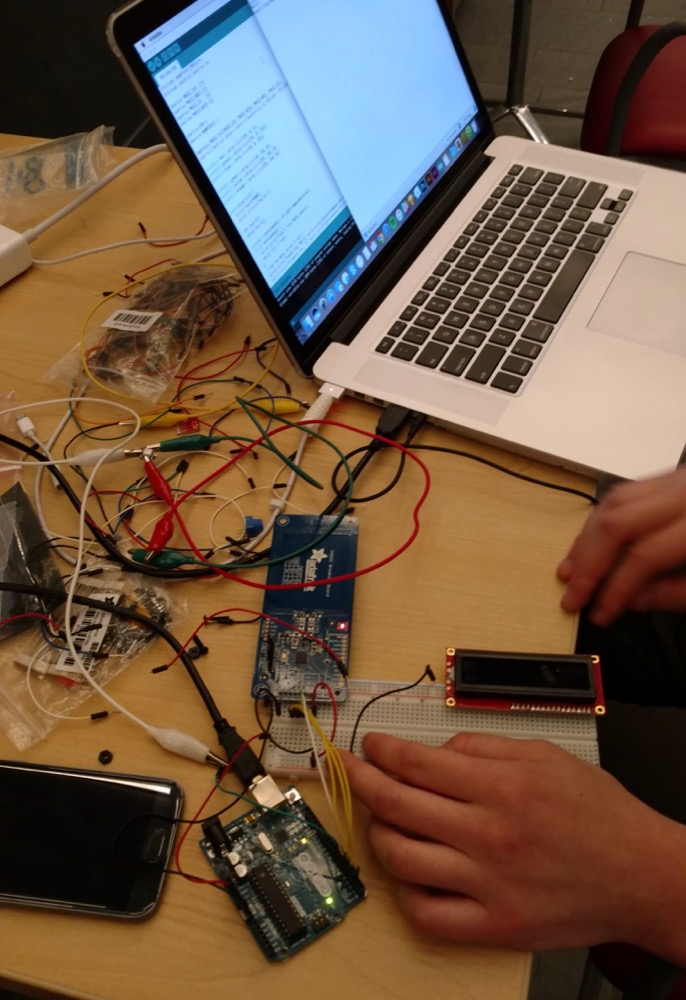
\includegraphics[width=\columnwidth]{debug}
\caption{The debugging of the system, and the testing of the wiring layout took
	place on an external breadboard.}
\label{fig:debug}
\end{figure}

The wiring layout was first tested on an external breadboard, to verify the
functionality of all the components independently, as depicted in Figure~\ref{fig:debug}.
Once all the components were working in harmony, the circuit was reassembled on a
breadboard which was affixed to the bottom of the prototype box.

\begin{figure}[!ht]
\centering
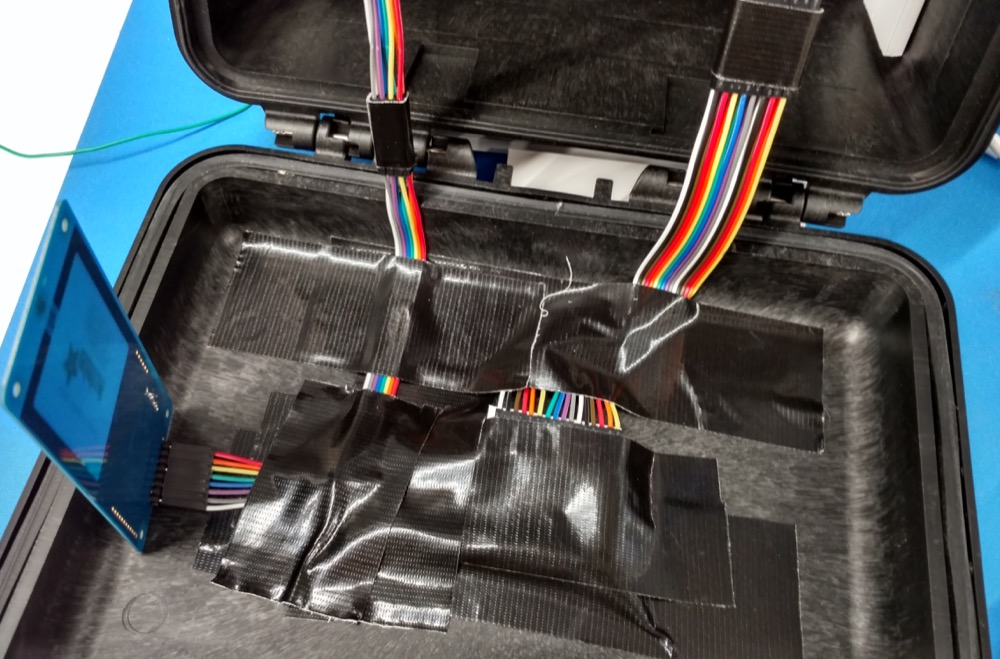
\includegraphics[width=\columnwidth]{box_lid}
\caption{The lid of the box, before the foam was added, showing the LCD Display
	(covered in tape) and the RFID sensor (the blue board to the left), and their
    associated ribbon cables connecting them to the rest of the circuitry.}
\label{fig:lid}
\end{figure}

Once a window was added to the lid of the box, the LCD Display was affixed beneath
it, and fastened in place. The RFID sensor was attached above, using standoffs to
make it flush with the rest of the lid, as depicted in Figure ~\ref{fig:lid}.
Once this subassembly was tested, the lid was padded with foam for additional
protection for the electronics and the box contents.

With the hardware then finished, the false bottom of the box was covered with
configurable foam, and the medications were added. The code was then finalized
and tested in preparation for the demo, whose configuration is visible in
Figure~\ref{fig:demo}.


\section{Medications} \label{meds}
While our prototype system can handle a wide range of different medications, each
subject to different constraints, we chose to use four common medications in our
demo system, each of which is a very common basic-life-support medications which can
be administered in most states at the EMT-Basic level of care.

\begin{center}
\captionof{table}{A table detailing the medications used in our demo prototype.}
\label{tab:meds} 
\begin{tabular}{|m{22em}|}
 \hline

 \textbf{Albuterol} (Ventolin) --- treats Asthma\\
 \hline
 Albuterol is a bronchodilator that is administered by a nebulizer, in conjunction
 with oxygen. Albuterol is sensitive to light.\\
 \hline\hline
 
 \textbf{Epinephrine} (EpiPen) --- treats Anaphylaxis\\
 \hline
 Epinephrine is a vasoconstrictor and a bronchodilator and can reverse allergic
 anaphylaxis. It is temperature sensitive.\\
 \hline\hline
 
 \textbf{Aspirin} (Bayer) --- treats Cardiac Chest Pain\\
 \hline
 Aspirin prevents blood from clotting and is indicated in individuals with a
 suspected myocardial infarction.\\
 \hline\hline
 
 \textbf{Oral Glucose} (Insta-Glucose) --- treats Hypoglycemia\\
 \hline
 Oral Glucose is a fast-acting sugar that is quickly absorbed into the blood and
 can reverse hypoglycemia and diabetic shock in diabetics.\\
 \hline
\end{tabular}
\end{center}


\section{System Performance \& Evaluation} \label{eval}
In addition to the informal testing which occurred during prototype design and
during the demo, the functionality of SmartBag was also tested more rigorously.
Starting with only a single item within the system, we tested the system's
ability to accurately track as many as 6 items simultaneously, and uncovered no
issues. The system always successfully monitored temperature and expiration
constraints; the only source of errors was the occasional RFID-read error, which
became more common as more items were added to the bag. Because each medication
is read frequently, these read errors never resulted in the system losing accuracy,
however, we suspect that these read errors will be the greatest limitation of the
prototype's ability to scale to implementations with many more items. Despite these
difficulties, we were able to achieve a system that achieved the primary design goals
for the project, and through testing, learn the greatest weaknesses of the system
to inform further refinement.

\begin{center}
\captionof{table}{Number of read errors for a given number of items within the bag.}
\label{tab:results} 
\begin{tabular}{|c|c|c|c|}
 \hline
 \# of Items & Loop Iterations & \# of Errors & Success Rate \\
 \hline
 1 & 99  & 0 & 100\%  \\
 2 & 100 & 0 & 100\%  \\
 3 & 100 & 1 & 99.0\% \\
 4 & 102 & 1 & 99.0\% \\
 5 & 101 & 2 & 98.0\% \\
 6 & 103 & 4 & 96.1\% \\
 \hline
\end{tabular}
\end{center}

Experimental results are depicted in Table~\ref{tab:results}. For each number of items,
we added the items to the box in a typical layout, and let the software loop run for a
number of iterations. The number of read errors encountered was then recorded.


\section{Future Improvements} \label{future}
While we believe that our system offers a great detail of utility in its current
state, a number of additional features or refinements would address some of the
issues mentioned in the previous section.

\begin{itemize}
\item Wireless Internet access, via either WiFi or a cellular data connection,
	would enable the transmission of alerts to the user. Alerts could be provided
	for numerous situations: 
	\begin{itemize}
	\item The temperature of the bag is approaching a dangerous point. 
	\item A medication will expire soon. 
	\item An item has expired or exceeded its environmental constraints. 
	\item An item is missing and needs to be resupplied before another call.
	\end{itemize}

\item A dedicated Android application for adding items to inventory would make
	for a substantial improvement in the user experience. This app could use the phone’s
	camera to scan a medication, automatically note the medication type, expiration date,
	batch number, and write all the information to the RFID tag to be affixed to the
	medication. A phone app could also communicate with the bag to notify the
    user when the temperature is dangerously high or low, when items are missing
    or expired, and could conveniently format a list for the user to use during
    resupply.

\item A more powerful RFID antenna would enable the scanning of items from a greater
	distance, which would allow more items to be placed in the bag. Ideally, in a
    full-scale deployment, SmartBag would be able to track hundreds of medications
    at once, and so this is a high priority for future work. One could also envision
    a system with multiple antennas placed on different sides of the bag, and a
    single processor which integrates scans from the multiple antennas in order
    to achieve complete coverage of the bag contents.

\item With the addition of a lid sensor and a buzzer, the bag could audibly alert
	the user if the medication was no longer potent.
    
\item Collaborations with equipment manufacturers would could have RFID tags added
	to 	items at the factory, and pre-encoded with information like the item's
    expiration date, so they arrive at the user ready to add to the bag.
\end{itemize}


\section{Conclusion} \label{conclusion}
Even the relatively limited functionality of our first prototype makes it clear
that there is a great deal of potential for the automation of equipment management
for emergency medical services providers. Even a simple system could perform much
of the tedious, error-prone work of daily truck checks and resupply, so that
busy first-responders could focus on their primary responsibility of providing
quality patient care. While our prototype is promising, and effectively demonstrates
the core functionality of a fully-fledged SmartBag system, it is clear that a great
deal of work remains before such a system could be brought to market. It remains to
be demonstrated that the system is capable of tracking the hundreds of items in a
real EMS bag. A more polished user-interface is needed as well, ideally a phone
application which smooths out the process of initially encoding RFID tags with
information as items are added to the system. While partnerships with equipment
manufactures could reduce this burden in the long run, such partnerships would
require economies of scale which are very far off.

Finally, any system, before it could be adopted by health-care providers, who
are notoriously conservative and slow to embrace new technology, must be
thoroughly, thoroughly tested. A system would need to demonstrate extreme
durability, accuracy, and reliability.

Despite these challenges, however, we believe that SmartBag demonstrates the
very real possibility for the use of an automated equipment management system.
Although such a system would not be easy to develop, and there are very clear
challenges to doing so, we truly believe that such a system would have a
definitively positive effect on the emergency medical services industry. An
automated system could reduce human error, improving quality care, as well as
reducing the stresses and cognitive loads placed on EMS care providers, a
group which is already overworked in many EMS systems.


\section{Acknowledgments} \label{acknowledgements}
We would like to thank:
\begin{itemize}
\item The Cornell Maker Club for the use of their lab space, tools, supplies,
	and training.
\item The staff of Cornell University Emergency Medical Services and Cornell
	Environmental Health and Safety for the donation of their supplies and
    expired medications for the construction of our prototype. 
\item The Cornell Rapid Prototyping Lab for the generous donation of time on their
	laser cutter.
\end{itemize}

% balance before bibliography
\balance

% If you want to use smaller typesetting for the reference list,
% uncomment the following line:
% \small
\bibliographystyle{acm-sigchi}
\bibliography{ubicomp}
\end{document}
